\mysubsection{Message et communication asynchrone}

\ifbook{
  \mysubsubsection{Problématique de la communication asynchrone}
}

\ifslide{
  \begin{frame}{Problématique de la communication asynchrone}
    \begin{block}{Motivations}
      \begin{itemize}
        \item \textit{fire and forget}
        \item \textit{can't wait}
        \item \textit{producteur / consommateur}
      \end{itemize}
    \end{block}

    \begin{block}{Problématiques}
      \begin{itemize}
        \item gestion d'erreur
        \item gérer les queues
        \item persistance (ou non) des messages
      \end{itemize}
    \end{block}
  \end{frame}

  \begin{frame}{Message Oriented Middleware (MOM)}
    \begin{block}{Domaines}
      \begin{itemize}
        \item Publish/Subscribe %(pub/sub) : n producteurs, n consommateurs
        \item Point To Point (PTP)% : n producteurs, 1 consommateur
      \end{itemize}
    \end{block}

    \begin{center}
      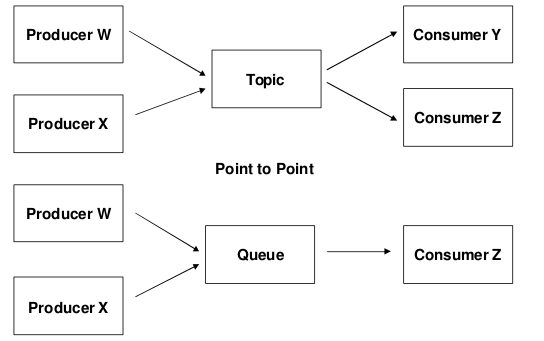
\includegraphics[scale=0.3]{img/topic-queue.png}
    \end{center}

  \end{frame}

  \begin{frame}
    \begin{block}{Invocation JMS}
      \begin{itemize}
        \item Localiser le driver JMS lookup JNDI. Le driver est une connection
factory
        \item Créer une connection JMS obtenir une connection à partir de la
connection factory
        \item Créer une session JMS :Il s'agit d'un objet qui va servir à recevoir et
envoyer des messages. On l'obtient à partir de la connection.
        \item Localiser la destination JMS: Il s'agit du canal sur lequel les
messages sont emis ou recus. Normalement, c'est réglé par le
déployeur. On obtient la destination via JNDI.
        \item Créer un producteur ou un consommateur JMS. Utilisés pour écrire
ou lire un message. On les obtient à partir de la destination et de la
session.
        \item Envoyer ou recevoir un message
      \end{itemize}
    \end{block}
  \end{frame}

  \begin{frame}{Message Oriented Middleware (MOM)}
    \begin{center}
      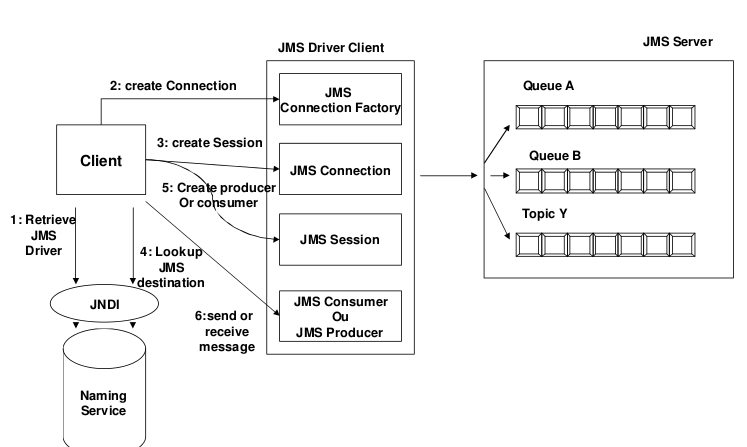
\includegraphics[scale=0.3]{img/jms-steps.png}
    \end{center}
  \end{frame}

  \begin{frame}{Message Oriented Middleware (MOM)}
    \begin{block}{Domaines}
      \begin{itemize}
        \item Transactions and MBD %: La production et la consommation du message sont dans deux transactions séparées...
        \item Sécurité %: Les MDB ne reçoivent pas les informations de sécurité du producteur avec le message.
      \end{itemize}
    \end{block}
  \end{frame}

  \begin{frame}
    \begin{block}{Advantages}
      \begin{itemize}
        \item message-based communications protocol
        \item store/buffer
        \item routing / load balancing
      \end{itemize}
    \end{block}
  \end{frame}

  \begin{frame}{Standardisation ?}
    \begin{block}{No Standard yet :( (API only) }
      \begin{itemize}
        \item JMS (Java Messaging System)
        \item MSMQ (Microsoft Message Queuing)
        \item Amazon Simple Queue Service
      \end{itemize}
    \end{block}

    \begin{block}{Protocol}
      \begin{itemize}
        \item AMQP (Advanced Message Queuing Protocol) - protocole
        \item STOMP (Streaming Text Oriented Messaging Protocol)
      \end{itemize}
    \end{block}
 \end{frame}
}

\demoframe{Communication Asynchrone}{
  Exemple avec JMS
}

